\documentclass{article}

\usepackage[utf8]{inputenc}
\usepackage[main=french]{babel}
\usepackage[T1]{fontenc}
\usepackage[export]{adjustbox}
\usepackage{csquotes}
\usepackage{graphicx}
\usepackage[acronym, toc, automake]{glossaries}

\makeglossaries
\makeindex

\newglossaryentry{taping}
{
    name=Taping,
    description={Toucher le pouce avec l'index}
}

\newglossaryentry{pull_test}
{
    name=Pull test,
    description={Consiste à tirer le patient vers soi afin de provoquer un déséquilibre pour observer sa réaction, ce qui permet d'évaluer les troubles liés à la maladie de Parkinson}
}

\newglossaryentry{bretteur}
{
    name=Man\oe{}uvre du bretteur,
    description={Elle consiste à tendre les bras en positionnant les deux index à quelques millimètres l’un de l’autre. Cela permet de déceler un éventuel tremblement d’attitude}
}

\newacronym{updrs}{UPDRS}{Unified Parkinson's Disease Rating Scale}

\newacronym{bvh}{BVH}{Biovision Hierarchy}

\newacronym{mocap}{MOCAP}{Motion capture}



\title{Protocole expérimental du projet E-mOove}
\date{19 Novembre 2020}
\author{Pierre Moreau\\
    \texttt{pierre.moreau@u-picardie.fr}\\
    \\
    \emph{Encadré par :}\\
    \\
    Jérôme Bosche\\
    \texttt{jerome.bosche@u-picardie.fr}\\ \and
    David Durand\\
    \texttt{david.durand@u-picardie.fr}
}

\begin{document}

\begin{figure}
    \centering
    
\includegraphics[height=0.14\textwidth]{img/Logo-UPJV-bleu.png}
    
\includegraphics[height=0.14\textwidth]{img/LogoMIS-BW.png}
    
\includegraphics[height=0.14\textwidth]{img/greco.jpg}
    
\includegraphics[height=0.14\textwidth]{img/elivie.png}
\end{figure}

\maketitle

\newpage

\tableofcontents

\newpage

\section{Introduction}

Le projet \textbf{E-mOove} est né d'une collaboration entre le laboratoire de Modélisation, Information et Systèmes (MIS) et l'unité CHIMERE au sein de l'institut GRECO, entre Michel Lefranc (CHIMERE/GRECO), Jérôme Bosche (MIS/GRECO) et David Durand (MIS/GRECO). L'objectif de ce projet est de pouvoir analyser, caractériser, classifier des mouvements en tout genre, dans les domaines du sport, de la musique ou encore de la santé. Chacun de ces domaines désire étudier les mouvements réalisés afin d'améliorer le geste, corriger des défauts ou faire apparaître les postures distinctives d'une pathologie. C'est d'ailleurs la maladie de Parkinson qui est le principal enjeux de ce projet, cette maladie neurovégétative entraîne des troubles de la mobilité. Actuellement, chaque patient doit se rendre à l'hôpital afin d'y être observé et filmé pendant qu'il effectue une série de mouvements et de postures décrites dans la section \ref{proc_chu}. Cette procédure est contraignante pour le patient qui doit se déplacer à l'hôpital et pour le diagnostique car les mouvements sont réalisés devant les médecins ce qui peut amener le patient à vouloir contrôler ses gestes. 

C'est pourquoi nous utilisons un dispositif de \acrshort{mocap} autorisant la récupération des données du patient après utilisation. Nous avons donc sélectionné la combinaison Perception Neuron Pro qui est composée de 17 capteurs sans fil permettant ainsi une installation simple. Ce dispositif peut donc être utilisée dans un milieu plus serein et moins stressant pour le patient (à son domicile). Les mouvements ainsi diversifiés et plus nombreux accorderont aux médecins plus d'aisance dans l'ajustement du traitement.

Ces données représentant la personne sous la forme d'un squelette en 3D (figure \ref{pnp}) seront exportées grâce au logiciel Axis Neuron Pro dédié à cette combinaison au format \acrshort{bvh}. Ainsi, nous disposons es données de positions et de rotations en 3 dimensions pour chacun des 17 capteurs de la combinaison. Ces données sont traitées grâce à des algorithmes qui exposeront les mouvements caractéristiques enregistrés.

\section{Le dispositif de capteurs}

\subsection{Perception Neuron Pro}

La combinaison Perception Neuron Pro (https://neuronmocap.com) est utilisé dans ce projet. Composée de 17 capteurs répartis sur le corps (figure \ref{pnp}), elle délivre 3 signaux de positions (px, py et pz) et 3 signaux de rotations (rx, ry et rz) par capteur. La hanche est le point repère de ce dispositif, elle contient toutes les données de déplacement dans l'espace de la personne. Les données des autres capteurs sont relatifs à ce point. Trois autres points du corps sont calculés par le logiciel : le cou et deux vertèbres. Finalement, 20 points composent le squelette, chacun d'entre eux délivre 6 signaux, on obtient alors 120 signaux pour le corps.

Dans la suite du projet, la combinaison Perception Neuron Studio sera utilisé afin de pouvoir capter les signaux des doigts, lesquels sont pertinents pour l'ajustement du traitement pour la maladie de Parkinson. Chaque main se décompose en 19 points (un sur chaque phalange) délivrant 6 signaux, on obtient alors un total de 114 signaux supplémentaires par main.

\begin{figure}
	\centering
	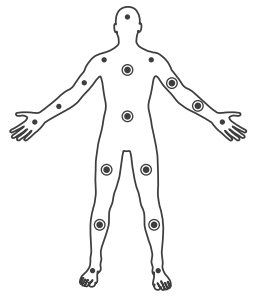
\includegraphics[scale=0.5]{img/17sensors.png}
	\caption{Perception Neuron Pro - 17 capteurs}
	\label{pnp}
\end{figure}

\subsection{Axis Neuron Pro}

Le logiciel Axis Neuron Pro (figure \ref{a_n_p}) retranscrit directement les mouvements effectués par l'utilisateur sur l'écran de l'ordinateur. Ce dernier récupère les données grâce à une antenne obtenue avec la combinaison. Lors d'un enregistrement de séquence, les données procurées par le logiciel sont au format brut, lequel n'est pas intuitif, ni utilisable directement avec nos algorithmes. C'est pourquoi nous exportons les données au format \acrshort{bvh}. Il est composé de deux sections : la première décrivant la hiérarchie et la pose initial du squelette, la seconde contenant les données des mouvements.

\begin{figure}
	\centering
	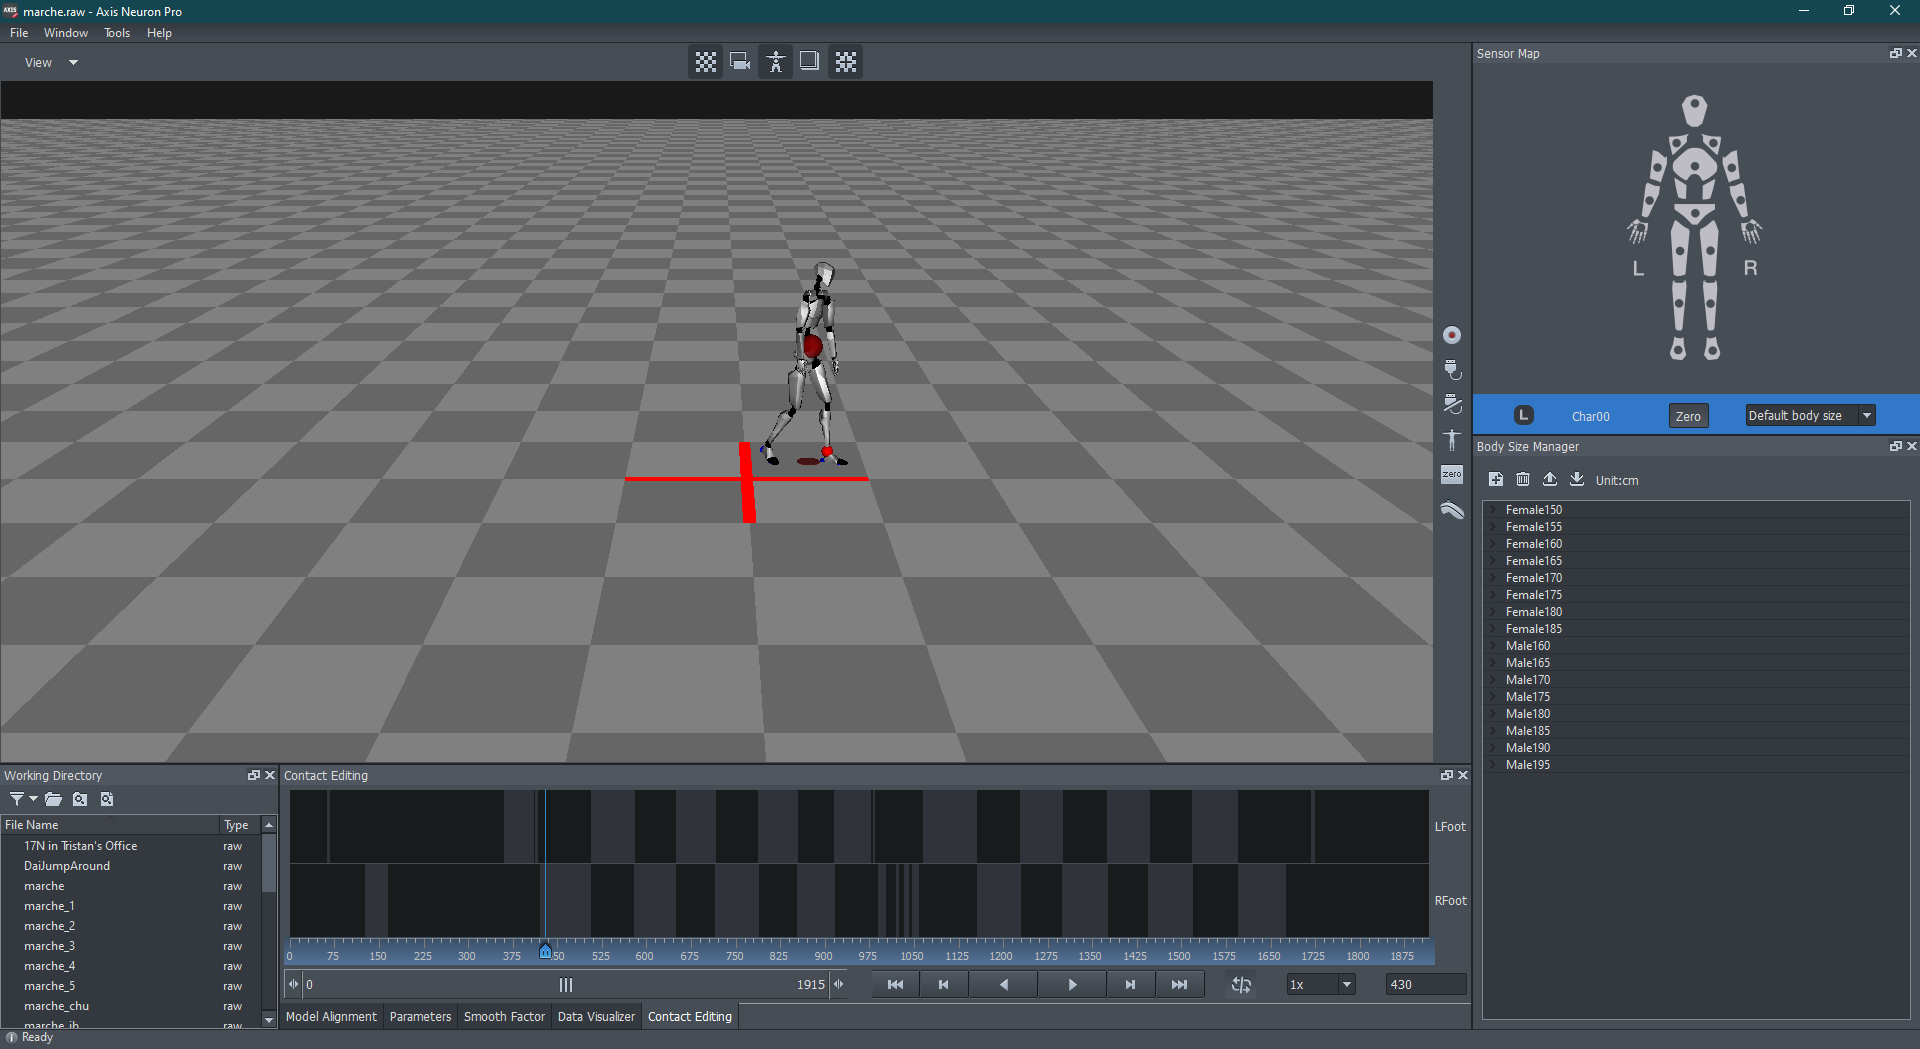
\includegraphics[scale=0.17]{img/axis_neuron_pro.png}
	\caption{Logiciel Axis Neuron Pro}
	\label{z_anp}
\end{figure}

Quelques pré-requis sur le logiciel sont nécessaire avant utilisation de la combinaison. Tout d'abord, les capteurs peuvent être calibrés dans leur boite (Tool $\longrightarrow$ Calibrate sensors). Cette étape n'est pas obligatoire mais doit être réalisée épisodiquement. Ensuite, 5 étapes admettent l'utilisation de la combinaison (figure \ref{z_anp}) :
\begin{enumerate}
	\item Connexion des capteurs au logiciel
	\item Sélection du sexe et de la taille de l'utilisateur : cela permet de savoir, approximativement, les dimensions de chaque membre du corps.
	\item Mise à zero du point de repère
	\item Calibration des capteurs grâce aux 3 poses T, A et S (figure \ref{poses})
	\item Enregistrement du mouvement : cela nécessite la sélection du nom de la scène enregistrée (section \ref{nommage_data}), puis un nouveau clique sur ce bouton arrête l'enregistrement
	\item Mets fin à la connexion des capteurs, permet aussi d'éteindre tous les capteurs
\end{enumerate}

\begin{figure}
	\centering
	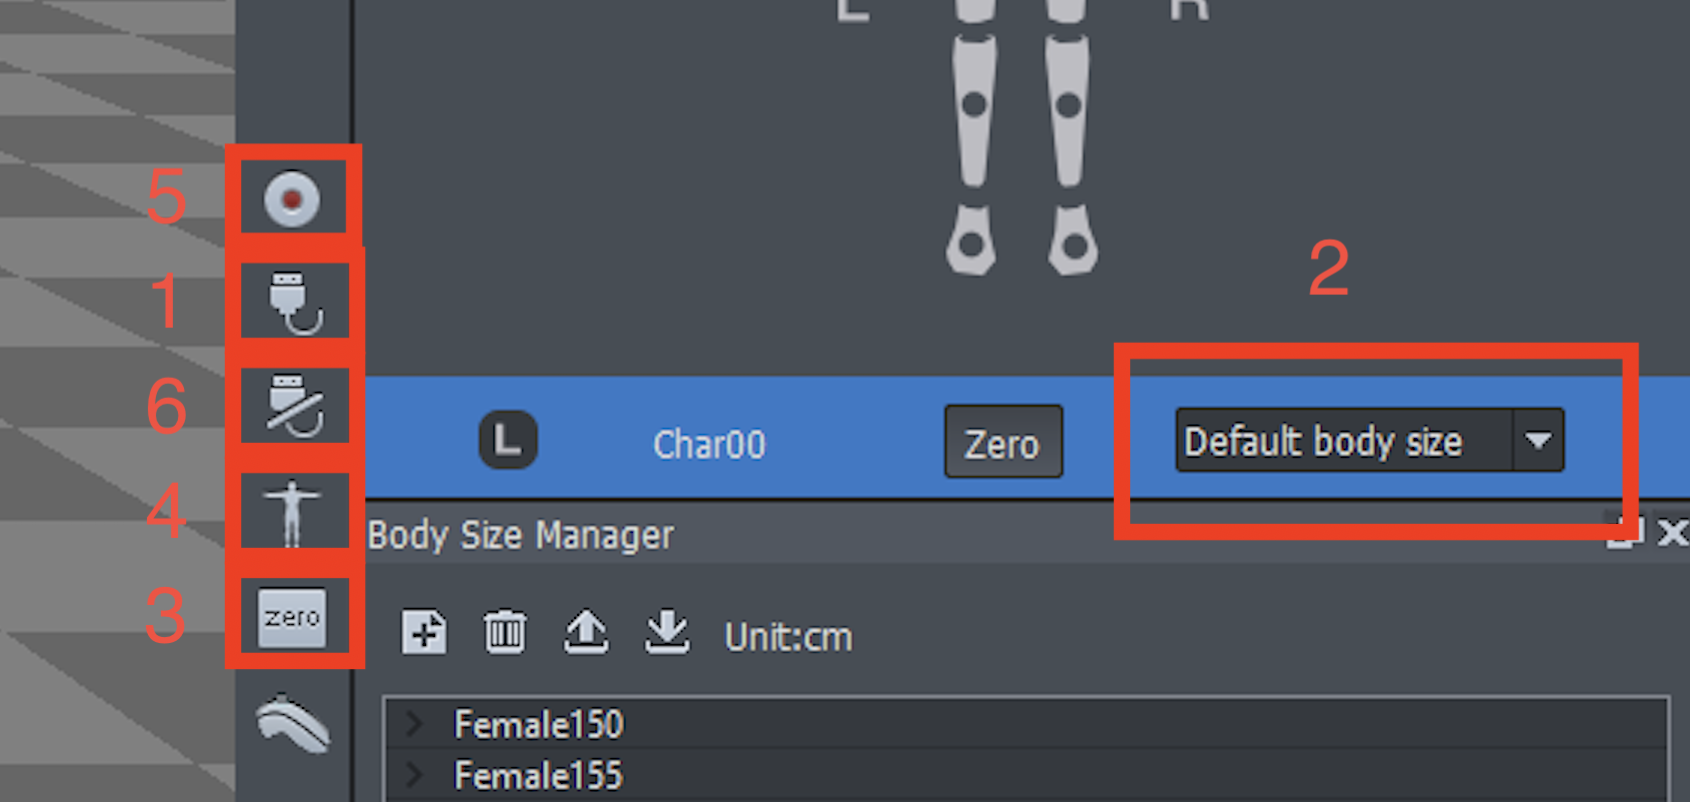
\includegraphics[scale=0.4]{img/zoom_anp.png}
	\caption{Logiciel Axis Neuron Pro}
	\label{a_n_p}
\end{figure}

\begin{figure}
	\centering
	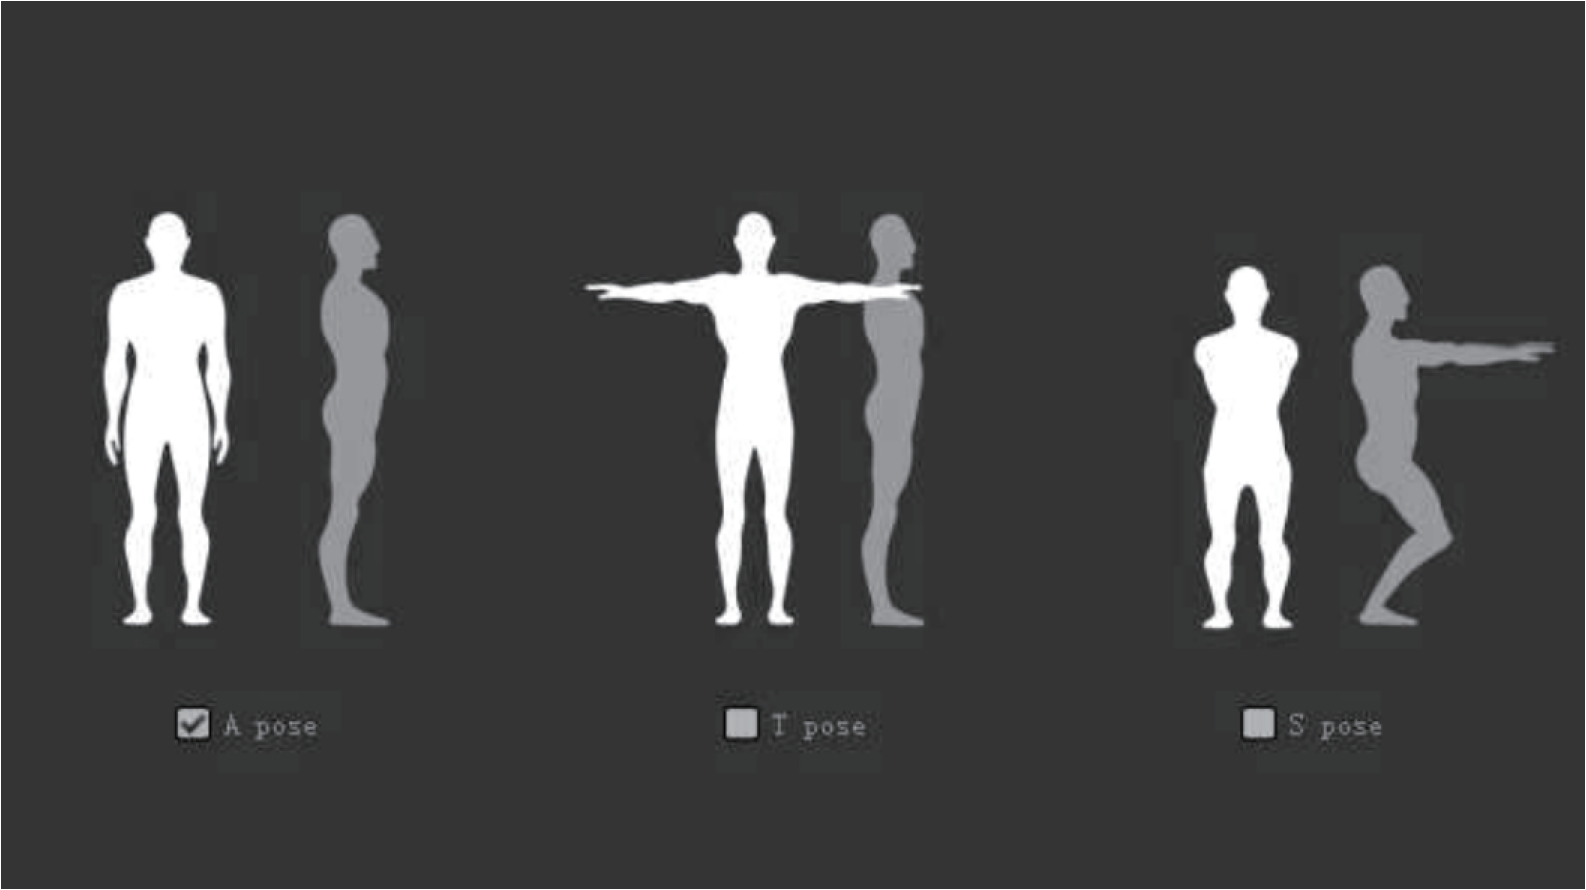
\includegraphics[scale=0.4]{img/poses.png}
	\caption{Poses A, T et S}
	\label{poses}
\end{figure}

\section{\acrlong{updrs}}

Cette échelle sert de mesure pour quantifier la progression de la maladie de Parkinson et l'efficacité du traitement. Elle contient 14 items côtés en 5 points de 0 (normal) à 4 (perturbation maximale). 

\begin{enumerate}
	\item Parole
	\item Expression faciale
	\item Tremblements au repos
	\item Tremblements d'action ou tremblement postural des mains
	\item Rigidité
	\item Tapotement des doigts 
	\item Mouvements des mains 
	\item Mouvements alternatifs rapides des mains
	\item Agilité de la jambe
	\item Se lever d'une chaise
	\item Posture
	\item Démarche
	\item Stabilité posturale
	\item Bradykinésie corporelle et hypokinésie
\end{enumerate}

\section{Enregistrement des données}
\label{nommage_data}

Afin de pouvoir sauvegarder toutes les données de toutes provenance, nous avons mis en place un système de nommage des fichiers. La création de la base de données est réalisée en deux phase (section \ref{protocole})., ce qui implique la séparation des données d'entraînement et de test dans deux dossiers. Plusieurs facteurs sont pris en compte :
\begin{enumerate}
	\item L'enregistreur (initial)
	\item L'utilisateur (01 pour valeur initiale)
	\item Essai (01 pour valeur initiale)
	\item Le numéro du mouvement exécuté (phase 1) / numéro de l'essai (phase 2) (01 pour valeur initiale) 
\end{enumerate}
Ces items sont ensuite joins les uns aux autres par un under-score dans l'ordre affiché.

\section{Procédure pour la réalisation de l'évaluation motrice au CHU d'Amiens}
\label{proc_chu}

La procédure exécutée au CHU d'Amiens se comporte différemment de la notre. Elle est réalisée par un patient atteint de la maladie de Parkinson et se déroule donc dans l'hôpital. 
\begin{enumerate}
	\item Se placer au bout couloir de l'hôpital
	\item Utiliser la chaise avec accoudoir 
	\item synchroniser l'enregistrement de la vidéo et du logiciel
	\item Réaliser la séquence motrice toujours dans le même ordre :
	\begin{enumerate}
		\item Faire parler le patient pour l'expression faciale et de la parole
		\item \Gls{taping} avec la main droite puis la gauche (10 fois)
		\item Ouverture et fermeture de la main droite puis de la main gauche (10 fois) 
		\item Mouvements alternatifs de la main droite puis de la gauche (rotation des poignets)
		\item Poser les bras sur les accoudoirs pour évaluer le tremblement au repos
		\item \Gls{bretteur} pour évaluer le tremblement postural
		\item Man\oe{}uvre doigt-nez pour évaluer le tremblement cinétique (10 fois)
		\item Agilité de la jambe droite puis de la gauche (10 fois)
		\item Mouvements du pied droit puis du gauche (10 fois)
		\item Laisser les membres inférieurs au repos pour évaluer le tremblement
		\item Lever de la chaise
		\item Marche aller-retour sur une distance de 7 mètres
		\item \Gls{pull_test} pour évaluer la posture 
	\end{enumerate}
	\item Une fois l'enregistrement terminé, évaluer les items de la rigidité
\end{enumerate}

\section{Description du protocole expérimentale}
\label{protocole}

Cette procédure considère deux étapes. Tout d'abord, chaque mouvement est réalisé puis enregistré dans l'ordre comme inscrit dans la procédure expliquée dans la section \ref{nommage_data}. Ces données labellisées permettrons l'entraînement des algorithmes.

Ensuite, 5 mouvements choisis aléatoirement sont effectués dans un ordre aléatoire, certains de ces mouvements peuvent être réalisés en parallèle. Cet enchaînement de mouvements sera précédé d'une marche sur une longueur de 2 mètres afin de pouvoir vérifier si les capteurs sont bien calibrés et avoir un point de référence.

\begin{enumerate}
	\item Marcher (10 pas)
	\item Demi-tour
	\item S'asseoir / Se lever
	\item S'asseoir / Se lever les mains sur les épaules
	\item Garde à vous
	\item Rotation du poignet bras tendu (10 fois / poignet)
	\item Toucher le nez avec l'index (10 fois)
	\item Taper le pied sur le sol (10 fois / pied)
	\item Lever de genou (10 fois / jambe)
	\item Applaudir
	\item Pas longs (5 fois)
	\item Équilibre sur un pied puis l'autre
	\item Reculer en marchant (10 pas)
	\item Monter / Descendre des escaliers
	\item Boire
	\item Lancer une balle
	\item Tremblement
	\item Freezing
	\item Regarder à gauche puis à droite
	\item Acquiescer
	\item Nier
	\item Test d'équilibre du Parkinson
\end{enumerate}

La combinaison utilisée actuellement ne concède pas  d'obtenir les données des phalanges mais le dispositif Perception Neuron Studio le permet. D'autres mouvements contenus dans la procédure du CHU pourront être ajoutés afin de compléter la base de données :

\begin{itemize}
	\item Taping 
	\item Ouverture et fermeture de la main droite puis de la main gauche (10 fois) 
\end{itemize}

\newpage
\printglossary
\printglossary[type=\acronymtype]

\end{document}